%Jennifer Pan, August 2011

\documentclass[10pt,letter]{article}
	% basic article document class
	% use percent signs to make comments to yourself -- they will not show up.

\usepackage{amsmath}
\usepackage{amssymb}
	% packages that allow mathematical formatting

\usepackage{graphicx}
	% package that allows you to include graphics

\usepackage{enumitem}

\usepackage{setspace}
	% package that allows you to change spacing

\onehalfspacing
	% text become 1.5 spaced

\usepackage{fullpage}
	% package that specifies normal margins

\renewcommand{\vector}[1]{\boldsymbol{#1}}
\newcommand{\problem}[1]{\section*{Problem #1}}
\newcommand{\problempart}[1]{\paragraph{#1}}

\begin{document}
	% line of code telling latex that your document is beginning


\title{Problem Set 3}

\author{Nicholas Wu}

\date{Fall 2020}
	% Note: when you omit this command, the current dateis automatically included

\maketitle
	% tells latex to follow your header (e.g., title, author) commands.
\textbf{Note:} I use bold symbols to denote vectors and nonbolded symbols to denote scalars. I primarily use vector notation to shorthand some of the sums, since many of the sums are dot products.

\problem{1}

\problempart{(1)}
\begin{enumerate}[label=(\alph*)]
\item We note that the absolute value is trivially nonnegative, and $|x-y| = 0$ implies $x=y$. Further, we have that the absolute value is symmetric, so $|x - y| = |y - x|$. Finally, we need to show the triangle inequality. Consider $x, y, z$. Then (using the facts that $|x| \ge x$ and $|x| \ge -x$)
\[ |x - y| + |y - z| \ge (x-y) + (y-z) \ge x-z\]
and
\[ |x - y| + |y - z| \ge (y - x) + (z - y) \ge z - x \]
Lastly, since $|x| \le \max(x, -x)$, we have that
\[ |x - y| + |y - z| \ge \max(z-x, x-z) \ge |x-z|\]
and so we have the triangle inequality. Hence $\rho$ is a metric space.
\item By definition, $\rho$ is nonnegative, and $\rho(x,y) = 0$ only when $x = y$. $\rho$ is also trivially symmetric: $\rho(x, y) = 1 = \rho(y, x)$ for $x \neq y$, and $\rho(x,x) = \rho(x,x)$. Finally, we have:
If $x \neq y \neq z$,
\[ \rho(x,y) + \rho(y,z) = 2 > \rho(x, z) \]
If $x = y \neq z$,
\[ \rho(x,y) + \rho(y,z) = 1 \ge \rho(x,z) \]
And if $x = y = z$:
\[ \rho(x,y) + \rho(y,z) = 0 \ge \rho(x,z) \]
Hence in all cases we still have the triangle inequality. Thus $\rho$ is a metric.
\item We note that since $|x(t) - y(t)|$ is nonnegative, the metric is nonnegative. We note that if $\rho(x,y) = 0$, then by definition of $\rho$, $\max |x(t) - y(t)| = 0$, implying $x(t) - y(t) = 0$ everywhere, which means $x(t) = y(t)$ everywhere.

Now we argue symmetry. This follows due to symmetry of the absolute value:
\[ \rho(x,y) = \max |x(t) - y(t)| = \max |y(t) - x(t)| = \rho(y, x) \]
Lastly, we argue for the triangle inequality. Consider $\rho(x,y) + \rho(y,z)$. We have
\[ \rho(x,y) + \rho(y,z) = \max|x(t) - y(t)| + \max|y(t) - z(t)| \]
\[ \ge \max \left(|x(t) - y(t)| + |y(t) - z(t)| \right) \]
\[ \ge \max |x(t) - z(t)| = \rho(x,z) \]
And hence we have triangle inequality. So $\rho$ is a metric.

\item We know that since $|x(t) - y(t)| \ge 0$, $\rho(x,y) \ge 0$. Additionally, the only way for the integral $\int |x(t) - y(t)| = 0$ is if the integrand is 0 everywhere, since the integrand cannot be negative. Hence , if $\rho(x,y) = 0$, we have $|x(t) - y(t)| = 0 \implies x(t) = y(t)$.

For symmetry, we have another easy argument from symmetry of the absolute value difference:
\[ \rho(x,y) = \int |x(t) -y(t)| = \int | y(t) - x(t)| = \rho(y,x)  \]

Lastly, using linearity of integration and triangle inequality on absolute value we argued for earlier,
\[ \rho(x,y) + \rho(y,z) = \int |x(t) - y(t)| + \int |y(t) - z(t)| = \int \left(|x(t) - y(t)| + |y(t) - z(t)| \right)  \]
\[ \ge \int |x(t) - z(t)| = \rho(x,z) \]
And hence $\rho$ is a metric.

\item The argument that $\rho$ is a metric proceeds exactly as in part a. We note that expanding the domain of $S$ from integers to rational numbers does not change the behavior of the metric.

\item We have nonnegativity since $f$ is increasing, $f(0) = 0$, and the absolute value is always nonnegative. Hence $f(|x-y|)$ will always be nonnegative. Further, since $f$ is strictly increasing, we have that for any $a > 0$, $f(a) > f(0) = 0$. Hence, if $f(|x-y|) = 0$, we must have $|x-y| = 0$ and therefore $x = y$.

Symmetry follows from symmetry of differences under absolute value:
\[ \rho(x,y) = f(|x-y|) = f(|y-x|) = \rho(y,x) \]

Finally, we argue for triangle inequality. By strict concavity of $f$ and the fact that $f(0)=0$, for $a, b \ge 0$,
\[  f(a) + f(b) = f\left( \frac{a}{a+b}(a+b) \right) +f\left(\frac{b}{a+b}(a+b) \right)  \]
\[ \ge \frac{a}{a+b}f(a+b) + \frac{b}{a+b}f(0) + \frac{b}{a+b}f(a+b) + \frac{a}{a+b}f(0)  \]
\[ = f(a+b) \]
Therefore, by the identity above and by the fact that $f$ is increasing and the triangle inequality of absolute value we showed earlier,
\[ \rho(x,y) + \rho(y,z) = f(|x-y|) + f(|y-z|) \]
\[ \ge f(|x-y| + |y-z|) \]
\[ \ge f(|x-z|) = \rho(x,z) \]
and we are done. Hence $\rho$ is a metric on $\mathbb{R}$.
\end{enumerate}
\problempart{(2)}
Statement: If $(S, \rho)$ is a complete metric space, and $T:S \to S$ is a contraction mapping with modulus $\beta$, then
\begin{enumerate}[label=(\alph*)]
\item $T$ has exactly one fixed point $v$ in $S$
\item for any $v_0 \in S$, $\rho (T^n v_0, v) \le \beta^n \rho(v_0, v)$.
\end{enumerate}
Proof: Pick an arbitrary $x \in S$, and define the sequence $v_n = T^n x$, where $T^0 x = x$. We first argue that $\{ v_n \}$ is Cauchy. We first note that
\[ \rho(v_1, v_0) \le \beta^0 \rho(v_1, v_0) \]
Inductively, now suppose that for $n-1$, $\rho(v_{n}, v_{n-1}) \le \beta^{n-1} \rho(v_1, v_0)$. Then by contraction mapping,
\[ \rho(v_{n+1}, v{n}) = \rho(Tv_{n}, Tv_{n-1}) \le \beta \rho(v_n, v_{n-1}) \le \beta^n \rho(v_1, v_0) \]
Hence we know that by induction, for any arbitrary $n$, $\rho(v_{n+1}, v_n) \le \beta^n \rho(v_1, v_0)$. Now, for any $m > n$, we have by triangle inequality,
\[ \rho(v^m, v^n) \le \sum_{i=n}^{m-1} \rho(v_i, v_{i+1}) \]
\[ \le \sum_{i=n}^{m-1} \beta^i \rho(v_1, v_0) \]
\[ \le \sum_{i=n}^\infty \beta^i \rho(v_1, v_0) \]
\[ = \frac{\beta^n}{1-\beta} \rho(v_1, v_0)\]
Hence, for any $\epsilon$, we can pick an $n$ such that $\beta^n \le (1-\beta)\epsilon / (2  \rho(v_1, v_0)) $, and then for all $m, m' \ge n$, by the triangle inequality,
\[ \rho(v^m, v^{m'}) \le \rho(v^m, v^n) + \rho(v^n, v^{m'}) \]
\[ \le 2 \frac{\beta^n}{1-\beta} \rho(v_1, v_0)\]
\[ \le \epsilon \]
And hence $v_n$ is a Cauchy sequence.

Now, because $\{v_n \} $ is Cauchy, and $S$ is complete, the sequence converges: $v_n \to v$ for some $v \in S$. We claim $v$ is our fixed point. By the triangle inequality,
\[ \rho(Tv, v) \le \rho(Tv, T^n x) + \rho(T^n x, v) \]
By the contraction mapping property,
\[ \rho(Tv, v) \le \beta \rho(v, v_{n-1}) + \rho(v_n, v) \]
Since $v_n \to v$, we have that as $n \to \infty$, $\rho(v, v_{n+1}) \to 0$ and $ \rho(v_n, v) \to 0$. Hence, taking $n\to \infty$ we get
\[ \rho(Tv, v) \le \beta(0) + 0 = 0 \]
Then since $\rho$ is nonnegative, we must have $\rho(Tv, v) = 0$, so $v = Tv$. Hence $v$ is a fixed point.

To finish (a), we now argue that $v$ is unique. Pick some fixed point $v'$. Then
\[ \rho(Tv', Tv) = \rho(v', v) \]
But by contraction mapping property, $\rho(Tv', Tv) \le \beta \rho(v', v)$, so we have
\[ \rho(v', v) = \rho(Tv', Tv) \le \beta \rho(v', v) \]
\[ (\beta - 1) \rho(v', v) \ge 0 \]
But we know $\beta < 1$, so in order for this to be true, we must have
\[ \rho(v', v) \le 0 \]
But $\rho$ is nonnegative, so we must have $\rho(v', v) = 0$ and hence $v' = v$. Hence the only fixed point is $v$.

For part (b), we proceed by induction. We can trivially confirm that for $n=0$, $\rho(v_0, v) \le \beta^0 \rho(v_0, v)$. Suppose the inductive hypothesis holds for $n-1$. Then by the contraction mapping property, since $Tv = v$, we get
\[ \rho(T^n v_0, v) = \rho(T^n v_0, Tv) \le \beta \rho(T^{n-1} v_0, v) \le \beta (\beta^{n-1} \rho(v_0, v)) \]
where we used the inductive hypothesis in the last step.
This implies
\[\rho(T^n v_0, v) \le \beta^n \rho(v_0, v) \]
and we are done.

Now, we prove Theorem 3.3: \\
\textbf{Statement}: Let $X \subseteq \mathbb{R}^l$, and let $B(X)$ be the space of bounded functions $f:X \to \mathbb{R}$ under the sup norm. Let $T: B(X) \to B(X)$ be an operator satisfying:
\begin{enumerate}[label=(\alph*)]
\item $\forall f, g \in B(X)$ such that $f(x) \le g(x) \forall x\in X$, $(Tf)(x) \le (Tg)(x) \forall x \in X$.
\item $\exists \beta \in (0,1)$ such that $\forall f \in B(X), a \ge 0, x\in X$,
\[ (T(f + a))(x) \le (Tf)(x)+\beta a \]
\end{enumerate}
Then $T$ is a contraction with modulus $\beta$.

\textbf{Proof:}
Since
\[ \rho(f, g) = \sup_x |f(x) - g(x)| \]
\[  g(x) + \rho(f,g) = g(x) + \sup_x |f(x) - g(x)| \ge g(x) + \sup_x f(x) - g(x) \ge g(x) + (f(x) - g(x)) = f(x) \]
Symmetrically,
\[ f(x) + \rho(f, g) = f(x) + \sup_x |f(x) - g(x)| \ge f(x) + \sup_x g(x) - f(x) \ge f(x) + (g(x) - f(x)) = g(x)\]
Since this holds for all $x$, we can apply condition $(a)$ on $T$ to get:
\[ (T(g+ \rho(f,g)))(x) \ge (Tf)(x)  \]
\[ (T(f+ \rho(f,g)))(x) \ge (Tg)(x)  \]
Applying condition 2, we have
\[ (Tg)(x) + \beta \rho(f,g) \ge (T(g+ \rho(f,g)))(x) \ge (Tf)(x)  \]
\[ (Tf)(x) + \beta \rho(f,g) \ge (T(f+ \rho(f,g)))(x) \ge (Tg)(x)  \]
Rearranging, we have
\[ (Tf)(x) - (Tg)(x) \le \beta \rho(f,g) \]
\[ (Tg)(x) - (Tf)(x) \le \beta \rho(f,g) \]
Then
\[ \sup_x |(Tf)(x) - (Tg)(x)| \le \beta \rho(f,g) \]
\[ \rho(Tf, Tg) \le \beta \rho(f,g) \]
and hence $T$ is a contraction mapping with modulus $\beta$.
\problempart{(3)}
\subparagraph{(4.6)} \textbf{Statement}: Let $X \subseteq \mathbb{R}^l$ be convex. Let the correspondence $\Gamma:X \to X$ be nonempty, compact-valued, and continuous. Define $A = \{(x,y)\in X \times X : y \in \Gamma(x) \}$. Let $F: A \to \mathbb{R}$ be continuous and bounded, and let $\beta \in (0,1)$. Let $C(X)$ be the space of continuous, bounded functions $X \to \mathbb{R}$ under the sup norm.

Then the operator $T$ defined as $Tf(x) = \max_{y \in \Gamma(x)} F(x,y) + \beta f(y)$ maps $C(X)$ into itself, has a unique fixed point $v \in C(X)$, and for all $v_0\in C(X)$,
\[ || T^n v_0 - v|| \le \beta^n || v_0 - v|| \]
Further, the optimal policy correspondence $G_v:X \to X $ defined by $G(x) = \{ y \in \Gamma(x) : \ v(x) = F(x,y)+\beta v(y) \} $ is compact-valued and continuous.

\textbf{Proof}:
We first show that for any $f \in C(X)$, $Tf$ is bounded and continuous. Note that since $F$ and $f$ are both bounded and $\Gamma$ is compact valued (and hence is bounded-valued), we have that $Tf$ must also be bounded. Also, since $F$ and $f$ are both continuous, and $\Gamma$ is compact-valued and continuous, by Berge's theorem of the maximum we know $Tf$ is continuous. Therefore, $Tf \in C(X)$ since it is bounded and continuous.

We now show $T$ satisfies the conditions for Theorem 3.3 that we proved in the previous problem part. We first check monotonicity. Suppose $f(x) \le g(x) \forall x$:
\[ (Tf)(x) = \max_{y \in \Gamma(x)} F(x,y) + \beta f(y) \le \max_{y \in \Gamma(x)} F(x,y) + \beta g(y) = (Tg)(x) \]
Now we show discounting:
\[ (T(f+a))(x) = \max_{y \in \Gamma(x)} F(x,y) + \beta (f(y) + a) = \max_{y \in \Gamma(x)} (F(x,y) + \beta f(y)) + \beta a \]
\[ \le (Tf)(x) + \beta a \]
Therefore, we know by Theorem 3.3 that $T$ is a contraction mapping with modulus $\beta$. By theorem 3.2 we proved in the previous problem, we have that $T$ has a unique fixed point $v \in C(X)$, and further that
\[ ||T^n v_0 - v|| \le \beta^n ||v_0 -v|| \]
for all $v_0 \in C(X)$.

Lastly, by Berge's theorem of the maximum, the maximizer correspondence $G$ is compact-valued and continuous.
\subparagraph{(4.7)} \textbf{Statement}: Let $X \subseteq \mathbb{R}^l$ be convex. Let the correspondence $\Gamma:X \to X$ be nonempty, compact-valued, continuous and monotone; for $x \le x'$, $\Gamma(x) \subseteq \Gamma(x')$. Define $A = \{(x,y)\in X \times X : y \in \Gamma(x) \}$. Let $F: A \to \mathbb{R}$ be continuous, bounded, and strictly increasing in its first $l$ arguments, and let $\beta \in (0,1)$. Then the solution to
\[ v(x) = \max_{y \in \Gamma(x)}(F(x,y)+ \beta v(y)) \]
is strictly increasing.

\textbf{Proof}: We know from theorem $4.6$ we proved previously that $v$ is the unique fixed point of $T$, which takes
\[(Tf)(x) = \max_{y \in \Gamma(x)} F(x,y) + \beta f(y) \]
Suppose $f$ is a nondecreasing function. Then if $x < x'$, since $F$ is strictly increasing in the first $l$ arguments,
\[ (Tf)(x) = \max_{y \in \Gamma(x)} F(x,y) + \beta f(y) < \max_{y \in \Gamma(x)} F(x',y) + \beta f(y)\]
Since $\Gamma$ is monotone,
\[ \max_{y \in \Gamma(x)} F(x',y) + \beta f(y) \le \max_{y \in \Gamma(x')} F(x',y) + \beta f(y) = (Tf)(x') \]
Hence $(Tf)(x) < (Tf)(x')$, so $(Tf)$ is strictly increasing. Hence, if we pick $v_0$ to be a strictly increasing function, we have the sequence $\{ T^n v_0 \}$ consists of nondecreasing functions, which is a closed set. Hence by theorem 3.2 we showed, the sequence converges to $v$, and by closure of the set of nondecreasing functions, we know $v$ is a nondecreasing function. However, $v = Tv$, so by what we showed, $Tv = v$ must be strictly increasing. Hence we are done.

\subparagraph{(4.8)} \textbf{Statement}: Let $X \subseteq \mathbb{R}^l$ be convex. Let the correspondence $\Gamma:X \to X$ be nonempty, compact-valued, and continuous. Define $A = \{(x,y)\in X \times X : y \in \Gamma(x) \}$. Let $F: A \to \mathbb{R}$ be continuous, bounded, and strictly concave, and let $\beta \in (0,1)$. Finally, let $\Gamma(x)$ be such that $\forall y \in \Gamma(x)$, $y'\in\Gamma x'$, $\theta y + (1-\theta)y' \in \Gamma(\theta x + (1-\theta)x')$. Then the solution to
\[ v(x) = \max_{y \in \Gamma(x)}(F(x,y)+ \beta v(y)) \]
and the corresponding maximizer
\[ G(x) = \{ y \in \Gamma(x) : \ v(x) = F(x,y) + \beta v(y) \} \]
are such that $v$ is strictly concave and $G$ is continuous and single-valued.

\textbf{Proof:} We know from theorem $4.6$ we proved previously that $v$ is the unique fixed point of $T$, which takes
\[(Tf)(x) = \max_{y \in \Gamma(x)} F(x,y) + \beta f(y) \]
Suppose $f$ is a weakly concave function. Let $y$ be such that $Tf(x) = F(x,y) + \beta f(y)$, $y'$ such that $Tf(x') = F(x',y'), \beta f(y')$
Then by concavity of $F$, since $\lambda y + (1-\lambda)y' \in \Gamma(\lambda x + (1-\lambda)x')$, we get
\[(Tf)(\lambda x + (1-\lambda) x') \ge F(\lambda x + (1-\lambda) x',\lambda y + (1-\lambda)y') + \beta f(\lambda y + (1-\lambda)y') \]
\[ > \lambda F(x,\lambda y + (1-\lambda)y') + (1-\lambda) F(x',\lambda y + (1-\lambda)y') + \beta f(\lambda y + (1-\lambda)y') \]
By weak concavity of $f$,
\[ \ge  \lambda F(x,y) + \lambda \beta f(y) + (1-\lambda) F(x',y) + (1-\lambda)\beta f(y) \]
\[ = \lambda(Tf)(x) + (1-\lambda)(Tf)(x') \]
Hence $Tf$ is strictly concave. By the same logic in theorem 4.8, if we pick a strictly concave $v_0$, we have the sequence $\{ T^n v_0 \}$ consists of weakly concave functions, which is a closed set. Hence by theorem 3.2 we showed, the sequence converges to $v$, and by closure of the set of weakly concave functions, we know $v$ is a weakly concave function. However, $v = Tv$, so by what we showed, $Tv = v$ must be strictly concave.

Finally, we must show $G$ is single valued. Suppose $y \neq y' \in G(x)$. Then
\[ v(x) = F(x, y) + \beta v(y) = F(x, y') + \beta v(y') \]
Then by strict concavity of $F$ and $v$, $y'' = (y' + y)/2$ must satisfy
\[ F(x, y'') + \beta v(y'') \ge \frac{1}{2}(F(x, y) + \beta v(y)) + \frac{1}{2}(F(x, y') + \beta v(y')) = v(x) \]
which contradicts the maximization of $v$. Hence, no such pair $y, y'$ exist, and therefore $G$ is single-valued. By the theorem of the maximum, $G$ is upper hemicontinuous, and since any upper hemicontinuous, single-valued correspondence is continuous, $G$ is continuous.
\problempart{(4)}
\begin{enumerate}[label=(\alph*)]
\item Let $f$ be bounded. We need to show $Tf$ is also bounded. Then
\[ Tf(x) = \max_{y \in \Gamma(x)} F(x,y) + \beta f(y) \]
Now, since $F$ is bounded, $f$ is bounded, and $\Gamma(x)$ is compact and hence also bounded, we must have $Tf(x)$ is also bounded for all $x$, so $Tf$ is bounded. Hence $T:B(X) \to B(X)$. We then confirm that if $f(x) \le g(x) \forall x$, then
\[ Tf(x) = \max_{y \in \Gamma(x)} F(x,y) + \beta f(y) \le \max_{y \in \Gamma(x)} F(x,y) + \beta g(y) = Tg(x) \]
so we have monotonicity. We then check discounting:
\[ (T(f+a))(x) = \max_{y \in \Gamma(x)} F(x,y) + \beta (f(y) + a) = \max_{y \in \Gamma(x)} (F(x,y) + \beta f(y)) + \beta a \]
\[ \le (Tf)(x) + \beta a \]
So we have both discounting and monotonicity, so we satisfy the Blackwell conditions, so by Theorem 3.3, $T$ is a contraction mapping, and by theorem 3.2, $T$ has a unique fixed point $v$, and for any $v_0\in B(X)$,
\[|| T^nv_0 - v|| \le \beta^n||v_0-v||\]
Lastly, we see by the theorem of the maximum that the maximizer correspondence $G$ is nonempty, since $\Gamma$ is finite-valued and nonempty.

\item It suffices to show $T_h$ is a contraction mapping. We do this by using the Blackwell condition and theorem 3.3. We first check monotonicity. Suppose $f(x) \le g(x) \forall x$. Then
\[ (T_hf)(x) = F(x, h(x)) + \beta f(h(x)) \le F(x, h(x)) + \beta g(h(x))= (T_hg)(x) \]
Now, we check discounting:
\[ (T_h(f+a))(x) = F(x, h(x)) + \beta (f(h(x)) + a) = F(x, h(x)) + \beta f(h(x)) + \beta a \le (T_hf)(x) + \beta a \]
Hence $T_h$ is a contraction mapping by theorem 3.3, and so it has a unique fixed point $w$.

\item Consider $w_n$. We have, $\forall x$,
\[ w_n(x) = F(x, h_n(x)) + \beta w_n(h_n(x)) \le \max_{y \in \Gamma(x)} F(x, y) + \beta w_n(y) = (Tw_n)(x) \]
Further, since $h_{n+1}(x) \in \arg \max_{y \in \Gamma(x)} F(x, y) + \beta w_n(y)$, we have that
\[ (Tw_n)(x) = \max_{y \in \Gamma(x)} F(x, y) + \beta w_n(y) = F(x, h_{n+1}(x)) + \beta w_n(h_{n+1}(x)) = (T_{h_{n+1}}w_n)(x)   \]
But $w_{n+1}(x) = F(x, h_{n+1}(x)) + \beta w_{n+1}(h_{n+1}(x))$, so
\[ (Tw_n)(x) = (T_{h_{n+1}}w_n)(x) \]
Since $w_n \le Tw_n$, we have by monotonicity,
\[ T_{h_{n+1}}w_n \le T_{h_{n+1}} (Tw_n) = T^2_{h_{n+1}}w_n \]
Repeating, we get
\[ T_{h_{n+1}}w_n  \le T^2_{h_{n+1}}w_n \le T^3_{h_{n+1}}w_n ... \le T^N_{h_{n+1}}w_n \]
Using the fact that we showed $T_{h_{n+1}}w_n = Tw_n$, we have
\[ Tw_n \le T^N_{h_{n+1}}w_n\]
for all $N$. But as $N \to \infty$, by contraction mapping theorem, the RHS approaces $w_{n+1}$. Hence we have
\[ Tw_n \le w_{n+1} \]
Now, we note that $T^N w_n \ge T^{N-1} w_{n} \ge ... \ge w_n $. Note that as $N \to \infty$, the LHS approaches $v$, by contraction mapping. Hence, $v \ge w_n$ for all $n$.
Now, by the monotonicity conditions we showed ($Tw_n \le w_{n+1}$ and $w_n \le Tw_n$),
\[ || v - w_n|| \le || v- Tw_{n-1} || \]
\[ \le || v - T^2w_{n-2}  || \]
\[ \le || v - T^nw_0  || \]
But by the contraction mapping theorem, $|| v - T^n w_0|| \le \beta^n ||v - w_0||$. So
\[ || v - w_n||  \le \beta^n ||v - w_0|| \]
Hence, for any $\epsilon$, we can always pick an $N$ such that $\beta^N ||v - w_0|| \le \epsilon$, and then for all $n\ge N$, $ ||v - w_n || \le \epsilon$. Hence $w_n$ converges to $v$, the unique fixed point of $T$ by contraction mapping.
\end{enumerate}
\problem{2}

\problempart{(1)}
Let us guess the value function has form:
\[ V(k) = m \log k + n \]
Then the maximization problem is
\[ \max \log(\theta k^\alpha - k') + \beta V(k') \]
\[ \max \log(\theta k^\alpha - k') + \beta m \log k' + \beta n \]
This problem has the FOC:
\[ \frac{\beta m }{k'}- \frac{1}{\theta k^\alpha - k'} = 0 \]
\[ \frac{\theta k^\alpha - k'}{k'} = \frac{1}{\beta m } \]
\[ \frac{\theta k^\alpha}{k'} = \frac{\beta m + 1}{\beta m } \]
\[ k' = \frac{\beta m \theta k^\alpha }{\beta m + 1} \]
Plugging this in, we get
\[  m \log k + n = \log\left(\theta k^\alpha - \frac{\beta m \theta k^\alpha }{\beta m + 1} \right) + \beta m \log \left(\frac{\beta m \theta k^\alpha }{\beta m + 1}\right) + \beta n \]
\[  m \log k + n = \log\left(\frac{\theta k^\alpha }{\beta m + 1} \right) + \beta m \log (\beta m) +  \beta m \log \left(\frac{\theta k^\alpha }{\beta m + 1}\right) + \beta n \]
\[ m \log k + n = (\beta m + 1)\log\left(\frac{\theta k^\alpha }{\beta m + 1} \right) + \beta m \log (\beta m) + \beta n \]
\[ m \log k + n = \alpha (\beta m + 1)\log k + (\beta m + 1)\log\left(\frac{\theta  }{\beta m + 1} \right)  + \beta m \log (\beta m) + \beta n \]
Matching the coefficient of $\log k$, we get
\[ m = \alpha (\beta m + 1) \]
\[ m - \alpha \beta m = \alpha  \]
\[ m = \frac{\alpha }{1 - \alpha \beta} \]
Last, we find $n$ by matching constant terms and using our expression for $m$:
\[ n = (\beta m + 1)\log\left(\frac{\theta  }{\beta m + 1} \right)  + \beta m \log (\beta m) + \beta n \]
\[ (1-\beta) n = \left(\frac{1}{1 - \alpha \beta}\right)\log\left(\theta(1-\alpha\beta)   \right)  + \frac{\alpha\beta}{1-\alpha\beta}  \log \left(\frac{\alpha\beta}{1-\alpha\beta}\right) \]
\[ (1-\beta)(1-\alpha\beta) n = \log \theta + \log(1-\alpha\beta)   + \alpha\beta \log \alpha\beta - \alpha\beta\log(1-\alpha\beta) \]
\[ (1-\beta)(1-\alpha\beta) n = \log \theta + (1-\alpha\beta)\log(1-\alpha\beta)   + \alpha\beta \log \alpha\beta \]
\[  n =\frac{ \log \left( \theta (1-\alpha\beta)^{1-\alpha\beta} (\alpha\beta)^{\alpha\beta}\right)}{(1-\beta)(1-\alpha\beta)} \]
All together, the value function is:
\[ V(k) = m \log k + n = \frac{\alpha }{1 - \alpha \beta}\log k + \frac{ \log \left( \theta (1-\alpha\beta)^{1-\alpha\beta} (\alpha\beta)^{\alpha\beta}\right)}{(1-\beta)(1-\alpha\beta)} \]
And the policy function is
\[ g(k) = k' = \frac{\beta m \theta k^\alpha }{\beta m + 1} =  \alpha\beta \theta k^\alpha \]
\problempart{(2)}
We could go ahead and prove contraction mapping (which guarantees unique steady state and convergence) but we present a simpler argument. Let $k_n$ be the sequence of capital choices, where $k_n = g(k_{n-1})$. We know from the previous part that the steady state is given by
\[ g(k_{ss})= \alpha\beta\theta k_{ss}^\alpha  = k_{ss} \]
We then note that
\[ \frac{k_n}{k_{ss}} = \frac{\alpha\beta\theta k_{n-1}^\alpha}{\alpha\beta\theta k_{ss}^{\alpha}} = \left(\frac{k_{n-1}}{k_{ss}} \right)^\alpha \]
Chaining this, we get
\[ \frac{k_n}{k_{ss}} = \left(\frac{k_0}{k_{ss}}\right)^{\alpha^n} \]
Since $\alpha < 1$, as $n\to \infty$, $\alpha^n \to 0$, and hence $k_n / k_{ss} \to (k_0/k_{ss})^0 = 1$. Therefore, as $n \to \infty$, the sequence $k_n$ approaches the steady state.
\problempart{(3)} Rewriting, we get
\[ V(k) = \max_{l, k'} \log (\theta k^\alpha l^{1-\alpha} - k') + \log(1-l) + \beta V(k') \]
We once again try $V(k) = m\log k + n$. We get
\[ \max_{l, k'} \log(\theta k^\alpha l^{1-\alpha} - k') + \log(1-l) + \beta m \log k' + \beta n \]
The FOCs are:
\[\frac{\beta m }{k'} - \frac{1}{(\theta k^\alpha l^{1-\alpha} - k')} = 0 \]
\[\frac{(1-\alpha)\theta k^\alpha l^{-\alpha}}{(\theta k^\alpha l^{1-\alpha} - k')} - \frac{1}{1-l} = 0 \]
Solving, the first one gives us
\[\frac{(\theta k^\alpha l^{1-\alpha} - k')}{k'} = \frac{1}{\beta m}  \]
\[ \frac{k'}{\theta k^\alpha l^{1-\alpha} } = \frac{\beta m}{1 + \beta m} \]
\[ k'  = \frac{\beta m\theta k^\alpha l^{1-\alpha}}{1 + \beta m} \]
The second gives
\[\frac{(1-\alpha)\theta k^\alpha }{(\theta k^\alpha l - k'l^\alpha)} = \frac{1}{1-l}  \]
Plugging in $k'$, we get
\[\frac{(1-\alpha)\theta k^\alpha }{\theta k^\alpha l - \frac{\beta m\theta k^\alpha l^{1-\alpha}}{1 + \beta m}l^\alpha} = \frac{1}{1-l}  \]
\[\frac{(1-\alpha)(1 + \beta m)}{l} = \frac{1}{1-l}  \]
\[\frac{1 }{(1-\alpha)(1 + \beta m)} = \frac{1-l}{l} = \frac{1}{l} - 1 \]
\[\frac{1 + (1-\alpha)(1 + \beta m)}{(1-\alpha)(1 + \beta m)} = \frac{1}{l} \]
\[ l = \frac{(1-\alpha)(1 + \beta m)}{1 + (1-\alpha)(1 + \beta m)} \]
\[ k' = \frac{\beta m\theta k^\alpha l^{1-\alpha}}{1 + \beta m}  \]
Plugging into the overall expression for $V(k)$, we get

\[ V(k) = \log \left(\theta k^\alpha l^{1-\alpha} - \frac{\beta m\theta k^\alpha l^{1-\alpha}}{1 + \beta m}\right) + \log(1-l) + \beta m \log \left(\frac{\beta m\theta k^\alpha l^{1-\alpha}}{1 + \beta m}\right) + \beta n \]
\[ m \log k + n = \log k^\alpha + \log \left(\frac{\theta l^{1-\alpha}}{1 + \beta m}\right) + \log(1-l) + \beta m \log \beta m + \beta m \log k^\alpha + \beta m \log \left(\frac{\theta l^{1-\alpha}}{1 + \beta m}\right) + \beta n \]
Matching the $\log k$ terms, we get
\[ m \log k = \log k^\alpha + \beta m \log k^\alpha \]
\[ m = \alpha + \alpha\beta m \]
\[ m = \frac{\alpha}{1-\alpha\beta} \]
\[ 1 + \beta m = \frac{1}{1-\alpha\beta}\]
Then our expression for $l$ becomes
\[ l = \frac{(1-\alpha)(1 + \beta m)}{1 + (1-\alpha)(1 + \beta m)} \]
\[ = \frac{(1-\alpha)}{(1-\alpha\beta) + (1-\alpha)} \]
We note that optimal labor choice is independent of capital. Our policy function is then

\[ g(k) = \frac{\beta m\theta k^\alpha l^{1-\alpha}}{1 + \beta m} = \beta \alpha \theta k^\alpha \left( \frac{(1-\alpha)}{(1-\alpha\beta) + (1-\alpha)}\right)^{1-\alpha}  \]

Lastly, we solve for the constant term in the value function.
\[ n = \log \left(\frac{\theta l^{1-\alpha}}{1 + \beta m}\right) + \log(1-l) + \beta m \log \beta m + \beta m \log \left(\frac{\theta l^{1-\alpha}}{1 + \beta m}\right) + \beta n \]
\[ n(1-\beta) = \log \left(\theta l^{1-\alpha}(1 - \alpha\beta)\right) + \log(1-l) + \beta m \log \beta m + \beta m\log \left(\theta l^{1-\alpha}(1-\alpha\beta)\right)  \]
\[ n(1-\beta)(1-\alpha\beta)=  \log \left(\theta l^{1-\alpha}(1 - \alpha\beta)\right) + (1-\alpha\beta)\log(1-l) + \alpha\beta \log \alpha \beta - \alpha \beta \log (1-\alpha\beta) \]
\[ n(1-\beta)(1-\alpha\beta)=  \log \theta + (1-\alpha) \log l + (1-\alpha\beta)\log(1-l) + \alpha\beta \log \alpha \beta + (1 - \alpha \beta) \log (1-\alpha\beta) \]

\[ =  \log \theta + (1-\alpha) \log \left ( \frac{(1-\alpha)}{(1-\alpha\beta) + (1-\alpha)}\right) + (1-\alpha\beta)\log\left ( \frac{(1-\alpha\beta)}{(1-\alpha\beta) + (1-\alpha)}\right) + \alpha\beta \log \alpha \beta + (1 - \alpha \beta) \log (1-\alpha\beta) \]
\[ =  \log \theta + (1-\alpha)\log(1-\alpha) - (2-\alpha-\alpha\beta) \log (2-\alpha - \alpha\beta)+ \alpha\beta \log \alpha \beta + 2(1 - \alpha \beta) \log (1-\alpha\beta) \]

\[ n(1-\beta)(1-\alpha\beta) =  \log \left( \frac{\theta (1-\alpha)^{1-\alpha}(\alpha\beta)^{\alpha\beta}(1-\alpha\beta)^{2-2\alpha\beta}}{(2-\alpha-\alpha\beta)^{2-\alpha-\alpha\beta}}\right)  \]
\[ n = \frac{1}{(1-\beta)(1-\alpha\beta)}\log \left( \frac{\theta (1-\alpha)^{1-\alpha}(\alpha\beta)^{\alpha\beta}(1-\alpha\beta)^{2-2\alpha\beta}}{(2-\alpha-\alpha\beta)^{2-\alpha-\alpha\beta}}\right)  \]
And so our value function is
\[ V(k) = \frac{1}{1-\alpha\beta} \log k + \frac{1}{(1-\beta)(1-\alpha\beta)}\log \left( \frac{\theta (1-\alpha)^{1-\alpha}(\alpha\beta)^{\alpha\beta}(1-\alpha\beta)^{2-2\alpha\beta}}{(2-\alpha-\alpha\beta)^{2-\alpha-\alpha\beta}}\right) \]
\problempart{(4)} See separate file for code. The analytical result in 3 matches the numerical result from running the code, as we can see in the figures. The value function iteration is straightforward; for the policy function, we need to derive the optimization conditions for $l$ given $c(k), k$ and the Euler condition. From our FOCs we have :
\[\frac{(1-\alpha)\theta k^\alpha l^{-\alpha}}{(\theta k^\alpha l^{1-\alpha} - k')} - \frac{1}{1-l} = 0 \]
Our optimization condition for $l$ is then:
\[(1-\alpha)\theta k^\alpha l^{-\alpha}(1-l) = c(k) \]
For the Euler condition, we derive from the envelope theorem:
\[ \frac{\partial V}{\partial k} = \frac{\alpha \theta k^{\alpha - 1}l^{1-\alpha}}{c(k)} \]
And hence the maximization FOC is:
\[ \frac{-1}{c(k)} + \beta \frac{\alpha \theta (k')^{\alpha - 1}l^{1-\alpha}}{\theta (k')^\alpha l^{1-\alpha} - k'} = 0 \]
So for our optimization,
\[ \frac{1}{c^{\text{new}}(k)} =  \frac{\beta\alpha \theta (k')^{\alpha - 1}l^{1-\alpha}}{c^{\text{old}}(k')} \]
\[ c^{\text{new}}(k) =  \frac{c^{\text{old}}(k')}{\beta\alpha \theta (k')^{\alpha - 1}l^{1-\alpha}} \]


\begin{figure}
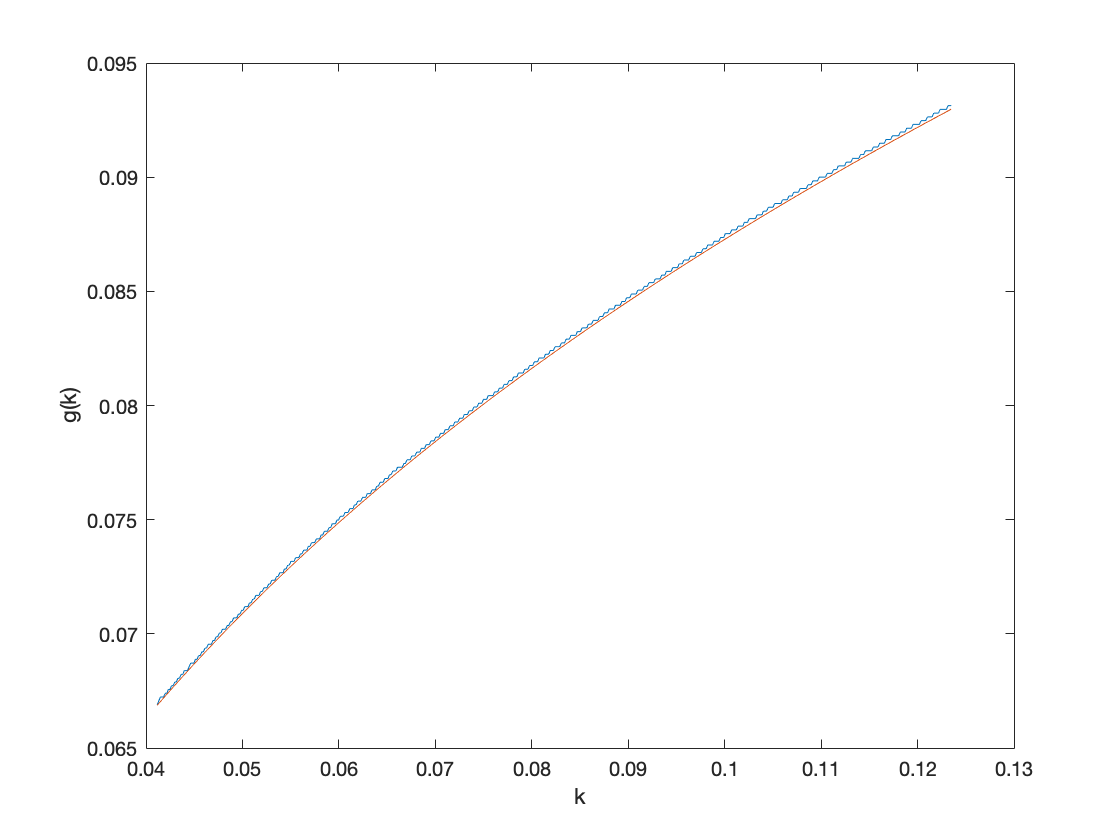
\includegraphics[scale=0.4]{ps3q2_valueiteration}
\caption{Value function iteration. Analytical result in red, numerical result in blue.}
\end{figure}
\begin{figure}
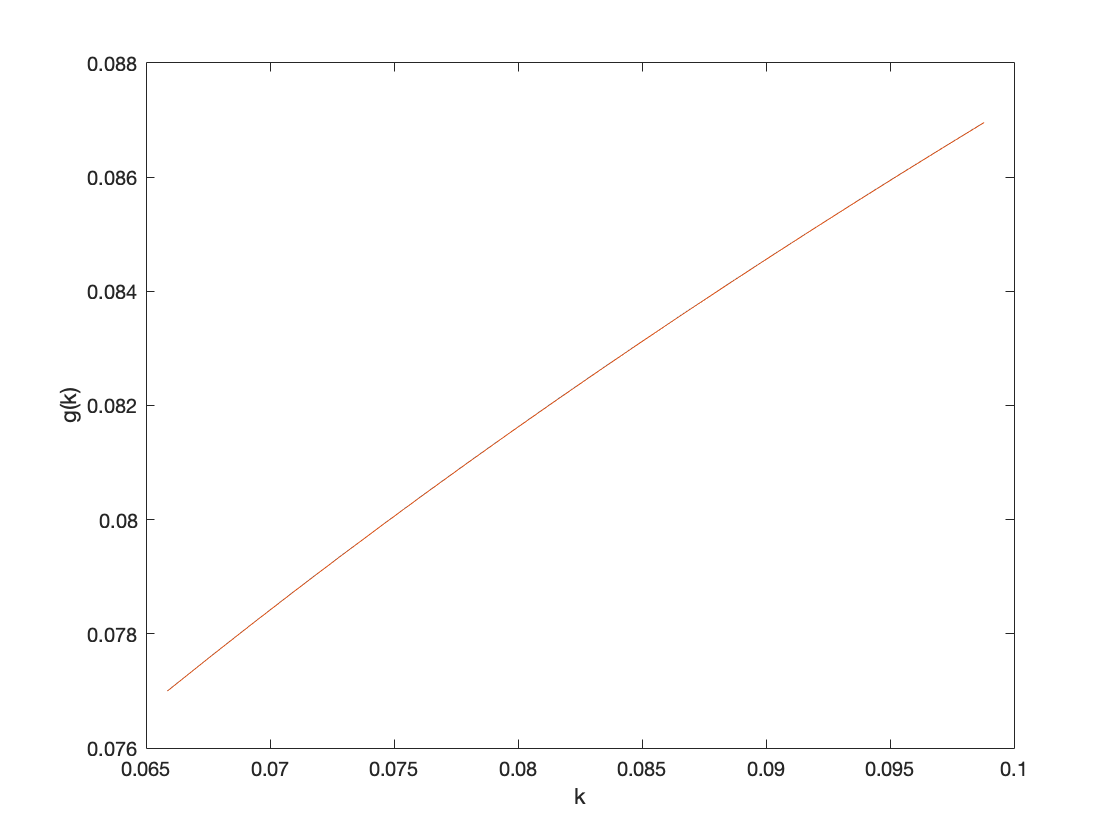
\includegraphics[scale=0.4]{ps3q2_policyiteration}
\caption{Policy function iteration. Analytical result in red, numerical result in blue. (These are super close, so they basically coincide)}
\end{figure}

\pagebreak

\problem{3}
\problempart{(1)}
By the Envelope theorem,
\[ \frac{\partial V}{\partial k_1} = \frac{\theta \alpha k_1^{\alpha-1}l_1^{1-\alpha} + (1-\delta_1)}{(\theta k_1^\alpha l_1^{1-\alpha} + (1-\delta_1)k_1 - k_1')^\sigma} \]
\[ \frac{\partial V}{\partial k_2} = \frac{\theta \mu k_2^{\mu-1}l_2^{1-\mu} + (1-\delta_2)}{(\theta k_2^\mu l_2^{1-\mu} + (1-\delta_2)k_2 - k_2')^\sigma} \]
Note we can substitute out $c_1$ and $c_2$ in terms of the respective $k_i, l_i, k'_i$, so we only have to worry about the constraint $l_1 + l_2 = 1$. Let $\lambda$ be the Lagrange multiplier on that constraint. Now, we have the maximization FOCs are, by taking partial derivatives with respect to $k'_1, k'_2, l_1, l_2$:
\[ - \frac{1}{(\theta k_1^\alpha l_1^{1-\alpha} + (1-\delta_1)k_1 - k_1')^\sigma} + \beta \frac{\partial V}{\partial k_1} = 0 \]
\[ - \frac{1}{(\theta k_2^\mu l_2^{1-\mu} + (1-\delta_2)k_2 - k_2')^\sigma} + \beta \frac{\partial V}{\partial k_2} = 0 \]
\[ \frac{(1-\alpha)\theta k_1^\alpha l_1^{-\alpha}}{(\theta k_1^\alpha l_1^{1-\alpha} + (1-\delta_1)k_1 - k_1')^\sigma}  - \lambda = 0 \]
\[  \frac{(1-\mu)\theta k_2^\mu l_2^{-\mu}}{(\theta k_2^\mu l_2^{1-\mu} + (1-\delta_2)k_2 - k_2')^\sigma} - \lambda = 0 \]
We can use the envelope theorem to plug in for the first two, and unify the last two to eliminate $\lambda$. Hence we get
\[ - \frac{1}{(\theta k_1^\alpha l_1^{1-\alpha} + (1-\delta_1)k_1 - k_1')^\sigma} + \beta \frac{\theta \alpha k_1^{\alpha-1}l_1^{1-\alpha} + (1-\delta_1)}{(\theta k_1^\alpha l_1^{1-\alpha} + (1-\delta_1)k_1 - k_1')^\sigma} = 0 \]
\[ - \frac{1}{(\theta k_2^\mu l_2^{1-\mu} + (1-\delta_2)k_2 - k_2')^\sigma} + \beta \frac{\theta \mu k_2^{\mu-1}l_2^{1-\mu} + (1-\delta_2)}{(\theta k_2^\mu l_2^{1-\mu} + (1-\delta_2)k_2 - k_2')^\sigma} = 0 \]
\[ \frac{(1-\alpha)\theta k_1^\alpha l_1^{-\alpha}}{(\theta k_1^\alpha l_1^{1-\alpha} + (1-\delta_1)k_1 - k_1')^\sigma} = \frac{(1-\mu)\theta k_2^\mu l_2^{-\mu}}{(\theta k_2^\mu l_2^{1-\mu} + (1-\delta_2)k_2 - k_2')^\sigma} \]
Making some simplifications, we get
\[ \frac{\beta \theta \alpha k_1^{\alpha-1}l_1^{1-\alpha} + \beta (1-\delta_1) - 1}{(\theta k_1^\alpha l_1^{1-\alpha} + (1-\delta_1)k_1 - k_1')^\sigma} = 0 \]
\[ \frac{\beta \theta \mu k_2^{\mu-1}l_2^{1-\mu} + \beta (1-\delta_2) - 1}{(\theta k_2^\mu l_2^{1-\mu} + (1-\delta_2)k_2 - k_2')^\sigma} = 0 \]
\[ \frac{(1-\alpha) k_1^\alpha l_1^{-\alpha}}{(\theta k_1^\alpha l_1^{1-\alpha} + (1-\delta_1)k_1 - k_1')^\sigma} = \frac{(1-\mu)\theta k_2^\mu l_2^{-\mu}}{( k_2^\mu l_2^{1-\mu} + (1-\delta_2)k_2 - k_2')^\sigma} \]
\problempart{(2)} See separate file.
\problempart{(3)} To compute the steady-states, we know
$(k_1^*)' = k_1^*$, $(k_2^*)' = k_2^*$. Then using the given parameter values, our FOCs can be written as
\[ \frac{\beta \alpha k_1^{\alpha-1}l_1^{1-\alpha} + \beta (1-\delta_1) - 1}{(k_1^\alpha l_1^{1-\alpha} -\delta_1 k_1 )^2} = 0 \]
\[ \frac{\beta \mu k_2^{\mu-1}l_2^{1-\mu} + \beta (1-\delta_2) - 1}{( k_2^\mu l_2^{1-\mu}  -\delta_2 k_2)^2} = 0 \]
\[ \frac{(1-\alpha) k_1^\alpha l_1^{-\alpha}}{( k_1^\alpha l_1^{1-\alpha} - \delta_1 k_1 )^2} = \frac{(1-\mu) k_2^\mu l_2^{-\mu}}{( k_2^\mu l_2^{1-\mu} -\delta_2 k_2 )^2} \]
From the first two, we get
\[\beta \alpha k_1^{\alpha-1}l_1^{1-\alpha} + \beta (1-\delta_1) = 1\]
\[ k_1^{\alpha-1}l_1^{1-\alpha}  = \frac{1 - \beta (1-\delta_1)}{\beta \alpha}\]
\[ \frac{l_1}{k_1}  = \left( \frac{1 - \beta (1-\delta_1)}{\beta \alpha} \right)^{\frac{1}{1-\alpha}}\]
\[ l_1  = k_1 \left( \frac{1 - \beta (1-\delta_1)}{\beta \alpha} \right)^{\frac{1}{1-\alpha}}\]
\[\beta \mu k_2^{\mu-1}l_2^{1-\mu} + \beta (1-\delta_2) = 1\]
\[k_2^{\mu-1}l_2^{1-\mu} = \frac{1 -\beta (1-\delta_2)}{\beta \mu} \]
\[ l_2 = k_2 \left( \frac{1 -\beta (1-\delta_2)}{\beta \mu} \right)^{\frac{1}{1-\mu}}\]
Before we finish, we make two notes that will simplify our calculations:
\[ k_1^\alpha l_1^{1-\alpha} = k_1 \left( \frac{1 - \beta (1-\delta_1)}{\beta \alpha} \right) \]
\[ k_2^\mu l_1^{1-\mu} = k_2 \left( \frac{1 -\beta (1-\delta_2)}{\beta \mu} \right) \]
so

\[ k_1^\alpha l_1^{1-\alpha} - \delta_1 k_1 = k_1 \left( \frac{1 - \beta (1-\delta_1)}{\beta \alpha}  - \delta_1\right) \]
\[ k_2^\mu l_1^{1-\mu} - \delta_2 k_2 = k_2 \left( \frac{1 -\beta (1-\delta_2)}{\beta \mu} - \delta_2 \right) \]
Now, we use the third FOC:
\[ \frac{(1-\alpha) k_1^\alpha l_1^{-\alpha}}{( k_1^\alpha l_1^{1-\alpha} - \delta_1 k_1 )^2} = \frac{(1-\mu) k_2^\mu l_2^{-\mu}}{( k_2^\mu l_2^{1-\mu} -\delta_2 k_2 )^2} \]
\[ \frac{(1-\alpha) \left( \frac{1 - \beta (1-\delta_1)}{\beta \alpha} \right)^{\frac{-\alpha}{1-\alpha}}}{k_1^2 \left( \frac{1 - \beta (1-\delta_1)}{\beta \alpha}  - \delta_1\right)^2} = \frac{(1-\mu) \left( \frac{1 -\beta (1-\delta_2)}{\beta \mu} \right)^{\frac{-\mu}{1-\mu}}}{k_2^2 \left( \frac{1 -\beta (1-\delta_2)}{\beta \mu} - \delta_2 \right)^2} \]
\[ \sqrt{\frac{(1-\alpha)  \left( \frac{1 -\beta (1-\delta_2)}{\beta \mu} \right)^{\frac{\mu}{1-\mu}}}{(1-\mu)\left( \frac{1 - \beta (1-\delta_1)}{\beta \alpha} \right)^{\frac{\alpha}{1-\alpha}}}} = \frac{k_1 \left( \frac{1 - \beta (1-\delta_1)}{\beta \alpha}  - \delta_1\right)}{k_2 \left( \frac{1 -\beta (1-\delta_2)}{\beta \mu} - \delta_2 \right)} \]
\[ \frac{k_1 }{k_2 } = \frac{\left( \frac{1 -\beta (1-\delta_2)}{\beta \mu} - \delta_2 \right)}{\left( \frac{1 - \beta (1-\delta_1)}{\beta \alpha}  - \delta_1\right)}\sqrt{\frac{(1-\alpha)  \left( \frac{1 -\beta (1-\delta_2)}{\beta \mu} \right)^{\frac{\mu}{1-\mu}}}{(1-\mu)\left( \frac{1 - \beta (1-\delta_1)}{\beta \alpha} \right)^{\frac{\alpha}{1-\alpha}}}}  \]
\[ \approx 0.653567 \]
Noting the labor constraint:
\[ l_1 + l_2 = 1 \]
\[ k_1 \left( \frac{1 - \beta (1-\delta_1)}{\beta \alpha} \right)^{\frac{1}{1-\alpha}} +k_2 \left( \frac{1 -\beta (1-\delta_2)}{\beta \mu} \right)^{\frac{1}{1-\mu}} = 1 \]
\[ k_2 \left((k_1/k_2)\left( \frac{1 - \beta (1-\delta_1)}{\beta \alpha} \right)^{\frac{1}{1-\alpha}} + \left( \frac{1 -\beta (1-\delta_2)}{\beta \mu} \right)^{\frac{1}{1-\mu}}\right) = 1\]
\[ k_2 = \frac{1}{(k_1/k_2)\left( \frac{1 - \beta (1-\delta_1)}{\beta \alpha} \right)^{\frac{1}{1-\alpha}} + \left( \frac{1 -\beta (1-\delta_2)}{\beta \mu} \right)^{\frac{1}{1-\mu}}}\]
\[ = \frac{1}{\frac{\left( \frac{1 -\beta (1-\delta_2)}{\beta \mu} - \delta_2 \right)}{\left( \frac{1 - \beta (1-\delta_1)}{\beta \alpha}  - \delta_1\right)}\sqrt{\frac{(1-\alpha)  \left( \frac{1 -\beta (1-\delta_2)}{\beta \mu} \right)^{\frac{\mu}{1-\mu}}}{(1-\mu)\left( \frac{1 - \beta (1-\delta_1)}{\beta \alpha} \right)^{\frac{\alpha}{1-\alpha}}}} \left( \frac{1 - \beta (1-\delta_1)}{\beta \alpha} \right)^{\frac{1}{1-\alpha}} + \left( \frac{1 -\beta (1-\delta_2)}{\beta \mu} \right)^{\frac{1}{1-\mu}}} \]
\[ = \frac{1}{\frac{\left( \frac{1 - 0.95 (1-0.08)}{0.95\cdot  0.5} - 0.08 \right)}{\left( \frac{1 - 0.95 (1-0.05)}{0.95 \cdot 0.36}  - 0.05\right)}\sqrt{\frac{(1-0.36)  \left( \frac{1 -0.95 (1-0.08)}{0.95 \cdot 0.5} \right)^{\frac{0.5}{1-0.5}}}{(1-0.5)\left( \frac{1 - 0.95 (1-0.05)}{0.95 \cdot 0.36} \right)^{\frac{0.36}{1-0.36}}}} \left( \frac{1 - 0.95 (1-0.05)}{0.95 \cdot 0.36} \right)^{\frac{1}{1-0.36}} + \left( \frac{1 -0.95 (1-0.08)}{0.95 \cdot 0.5} \right)^{\frac{1}{1-0.5}}} \]
\[ k_2 \approx 6.1597 \]
\[ k_1 = (k_1/k_2)k_2 \approx 4.0258 \]
\end{document}
	% line of code telling latex that your document is ending. If you leave this out, you'll get an error
